\documentclass[a4paper, 12pt]{article}

\usepackage{amsmath}
\usepackage[utf8]{inputenc}
\usepackage{graphicx}
\usepackage{caption}
\usepackage{physics}

\captionsetup{width=0.8 \linewidth}
\usepackage[parfill]{parskip}

\begin{document}

\title{\vspace{-4cm}Homework 1\\\large{FFR120 - Simulation of Complex Systems}\vspace{-0.7cm}}
\author{Vincent Udén\\udenv@student.chalmers.se}
\date{November - 2022}

\maketitle

\section*{Excercise 1.1}

\subsection*{a)}
Starting off with Newton's second law
\begin{equation} \label{eq:newton2}
    F = ma \iff m \dv[2]{r(t)}{t} = -r(t)k,
\end{equation}
one obtains a second order differential equation where the right hand side the force generated by a harmonic oscillator. This of course assumes that the point of equilibrium sits at $x_0 = 0$. This differential equation is solved by the trigonometric functions $\sin$ and $\cos$ since
\begin{equation}
    \dv[2]{\cos(\omega t)}{t} = -\omega^2 \cos(\omega t)
\end{equation}
and the same goes for $\sin$. If we add a phase shift $\phi$ and an amplitude $A$ to cosine we can cover the entire solution space with just
\begin{equation} \label{eq:sol}
    r(t) = A \cos(\omega t + \phi),
\end{equation}
since $\cos(t - \pi/2) = \sin(t)$. Finally we'll insert equation \eqref{eq:sol} into equation \eqref{eq:newton2}
\begin{equation}
    \dv[2]{(A \cos(\omega t + \phi))}{t} = - \frac{k}{m} r(t) \iff -A \omega^2 \cos(\omega t + \phi) = - \frac{k}{m} A \cos(\omega t + \phi),
\end{equation}
which results in two solutions where $\omega = \pm \sqrt{k/m}$. Since it doesn't matter I'll disregard the negative solution. $A$ and $\phi$ can be defined using an initial position $r_0$ and an initial velocity $v_0$ at $t=0$. This is done through the system of equations
\begin{equation}
    \begin{cases}
        r(0) = A \cos(\phi) = r_0 \\
        \dot{r}(0) = - A \omega \sin(\phi) = v_0.
    \end{cases}
\end{equation}
Reorganising these two equations, separating $\cos(\phi), \sin(\phi)$ and $A$ as described in the excercise results in
\begin{equation}
    \begin{cases}
        \cos(\phi) = \frac{r_0}{A} \\
        \sin(\phi) = -\frac{v_0}{A \omega} \\
        A^2(\cos^2(\phi) + \sin^2(\phi)) = r_0^2 + \frac{v_0^2}{\omega^2} \iff A = \pm \sqrt{r_0^2 + \frac{v_0^2}{\omega^2}},
    \end{cases}
\end{equation}
where the last equation comes from squaring the position and velocity equation before adding them. Note that this is not one unique solution since there are multiple axial symmetries and periodicity in the trigonometric functions.

\subsection*{b), c) \& d)}
The parameters used were $m=0.1, k=5, r_0=0.1, v_0=0$ resulting in $A=0.1,\phi=0,\omega=\sqrt{50}$. The characteristic frequency of this oscillator is $f=\omega/(2\pi) \approx 11.11$ Hz. If we convert the timesteps seen in figure \ref{fig:results} to frequencies ($f=1/\Delta t$) we obtain $f_1 = 10000, f_2 = 500, f_3 = 50$. Relative to the characteristic frequency these are about 1000, 50 and 5 times bigger. All of them diverge from the analytical solutions, just a different speeds. Therefore my conclusion is that no value of $\Delta t$ is really appropriate if the oscillator is to be ran forever.

\begin{figure}[h!]
    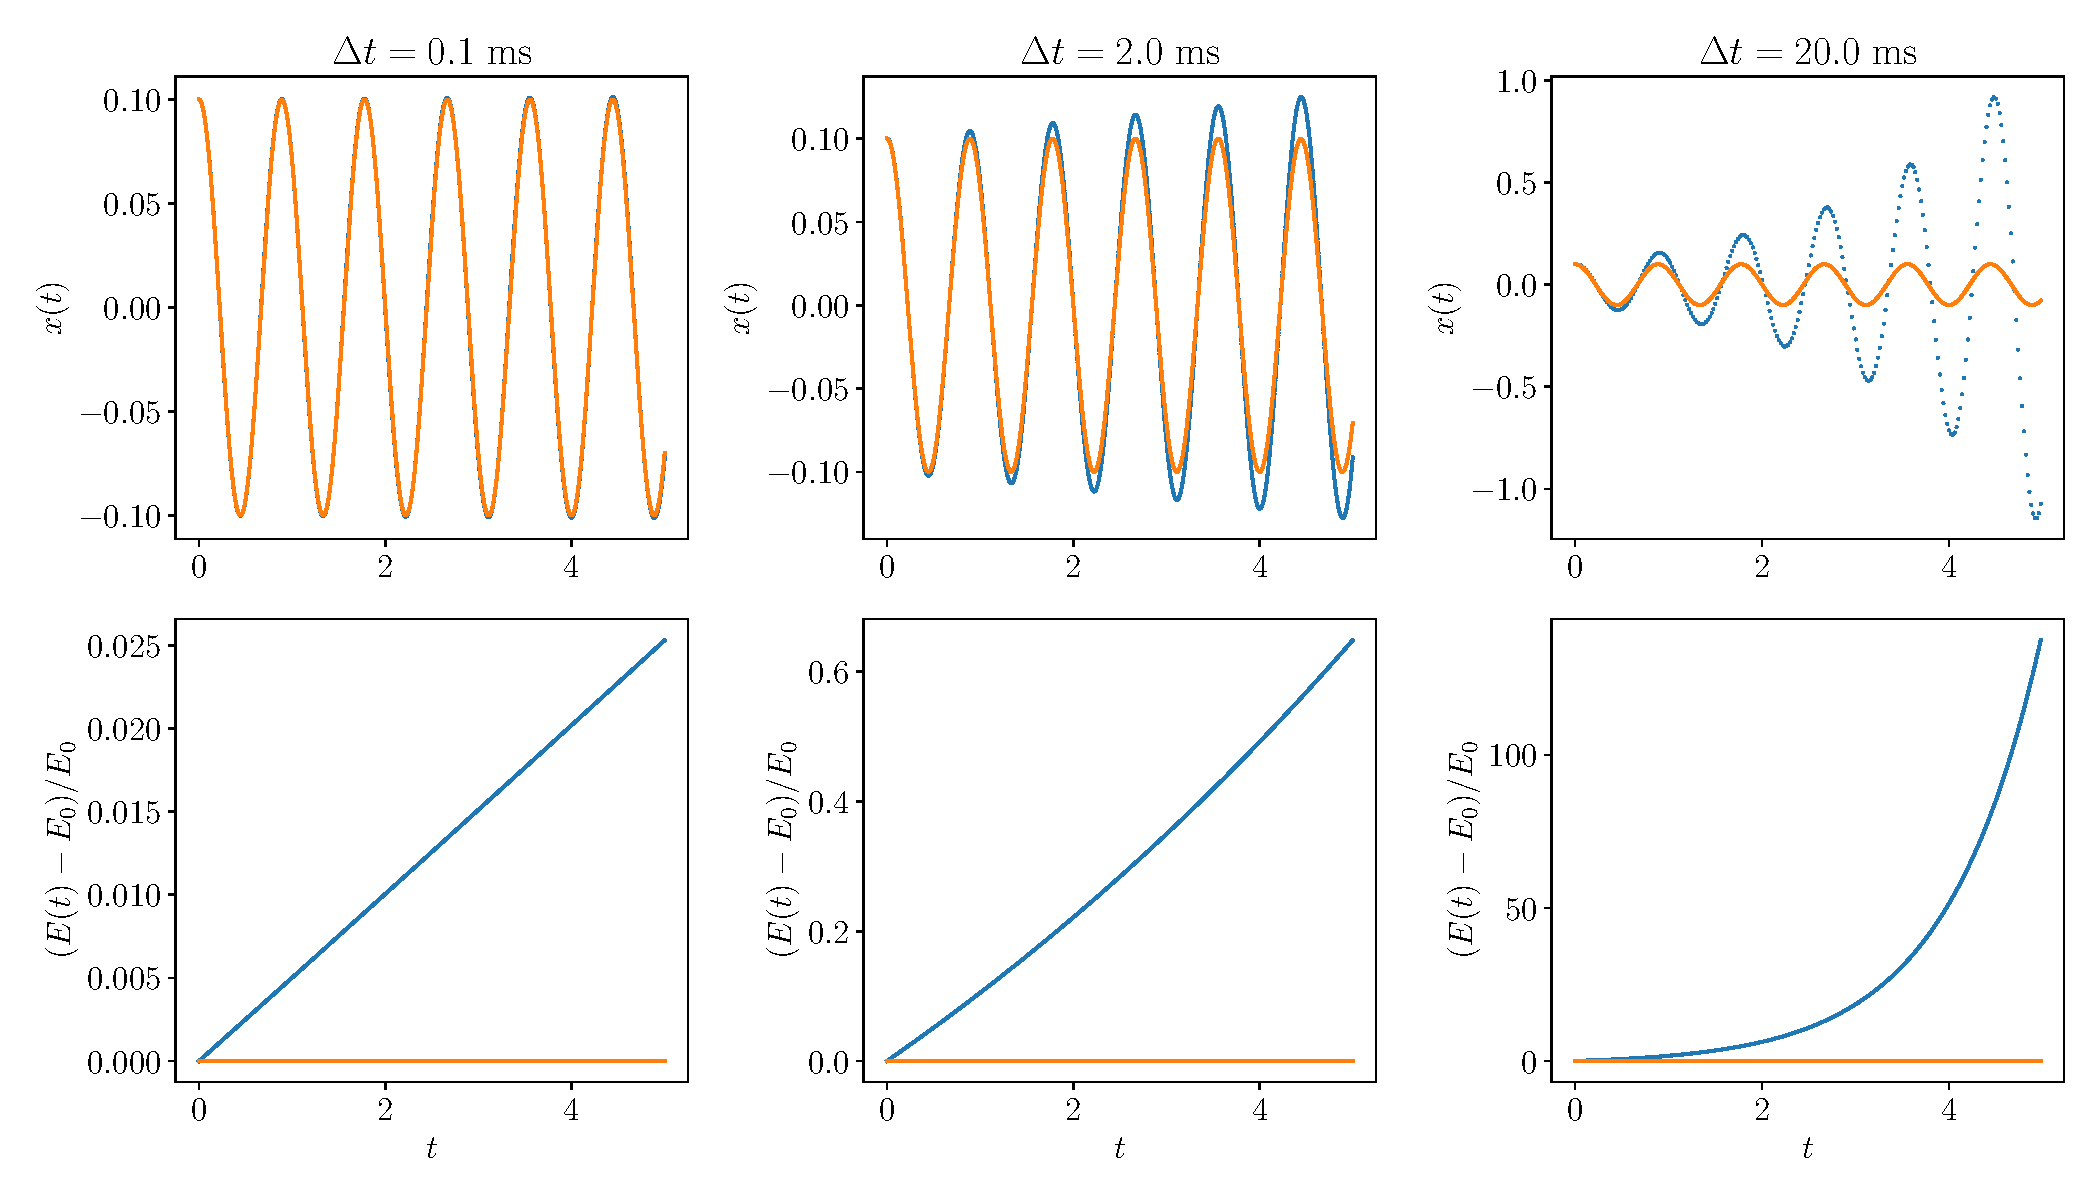
\includegraphics[width=\textwidth]{../Harmonic-Oscillator/figures/euler_forward.pdf}
    \caption{On the first row of plots the analytical path (orange line) and the numerical path (blue dots) for each column using a different timestep $\Delta t$. The second row does the same but for the relative deviation from the initial energy.}
    \label{fig:euler_results}
\end{figure}

The energies in figure \ref{fig:euler_results} show the same results as discussed in the previous paragraph. All timesteps results in increasing energy. This is to be expected as the Euler forward integration always lags behind an analytical solution. In this oscillatory case that results in the system turning back towards the equilibrium too late. If Euler backward integration were to be used instead the opposite problem would occur. The analytical solution doesn't stray at all from the initial energy of the system. If we were too zoom in incredibly far we'd of course spot a tiny floating point error but that isn't an error inherent to the method, it's just a limitation of finite memory.

\section*{Excercise 1.3}

\subsection*{a)}
The program is shown at the end of the report. It's the same program as for excercise 1.1, expect using the other integrator (leapfrog).

\subsection*{b \& c)}
The Leapfrog integration does a much better job at adhereing to the analytical trajectory. As can be seen in figure \ref{fig:leapfrog_results} the energies deviate as much as $0.5\%$. The important fact is that they're not drifting further and further away from the analytical solution. Even if restricted the the first period of the oscillator, the error for the same timestep is thousands of times smaller than that of the Euler method.

\begin{figure}[h!]
    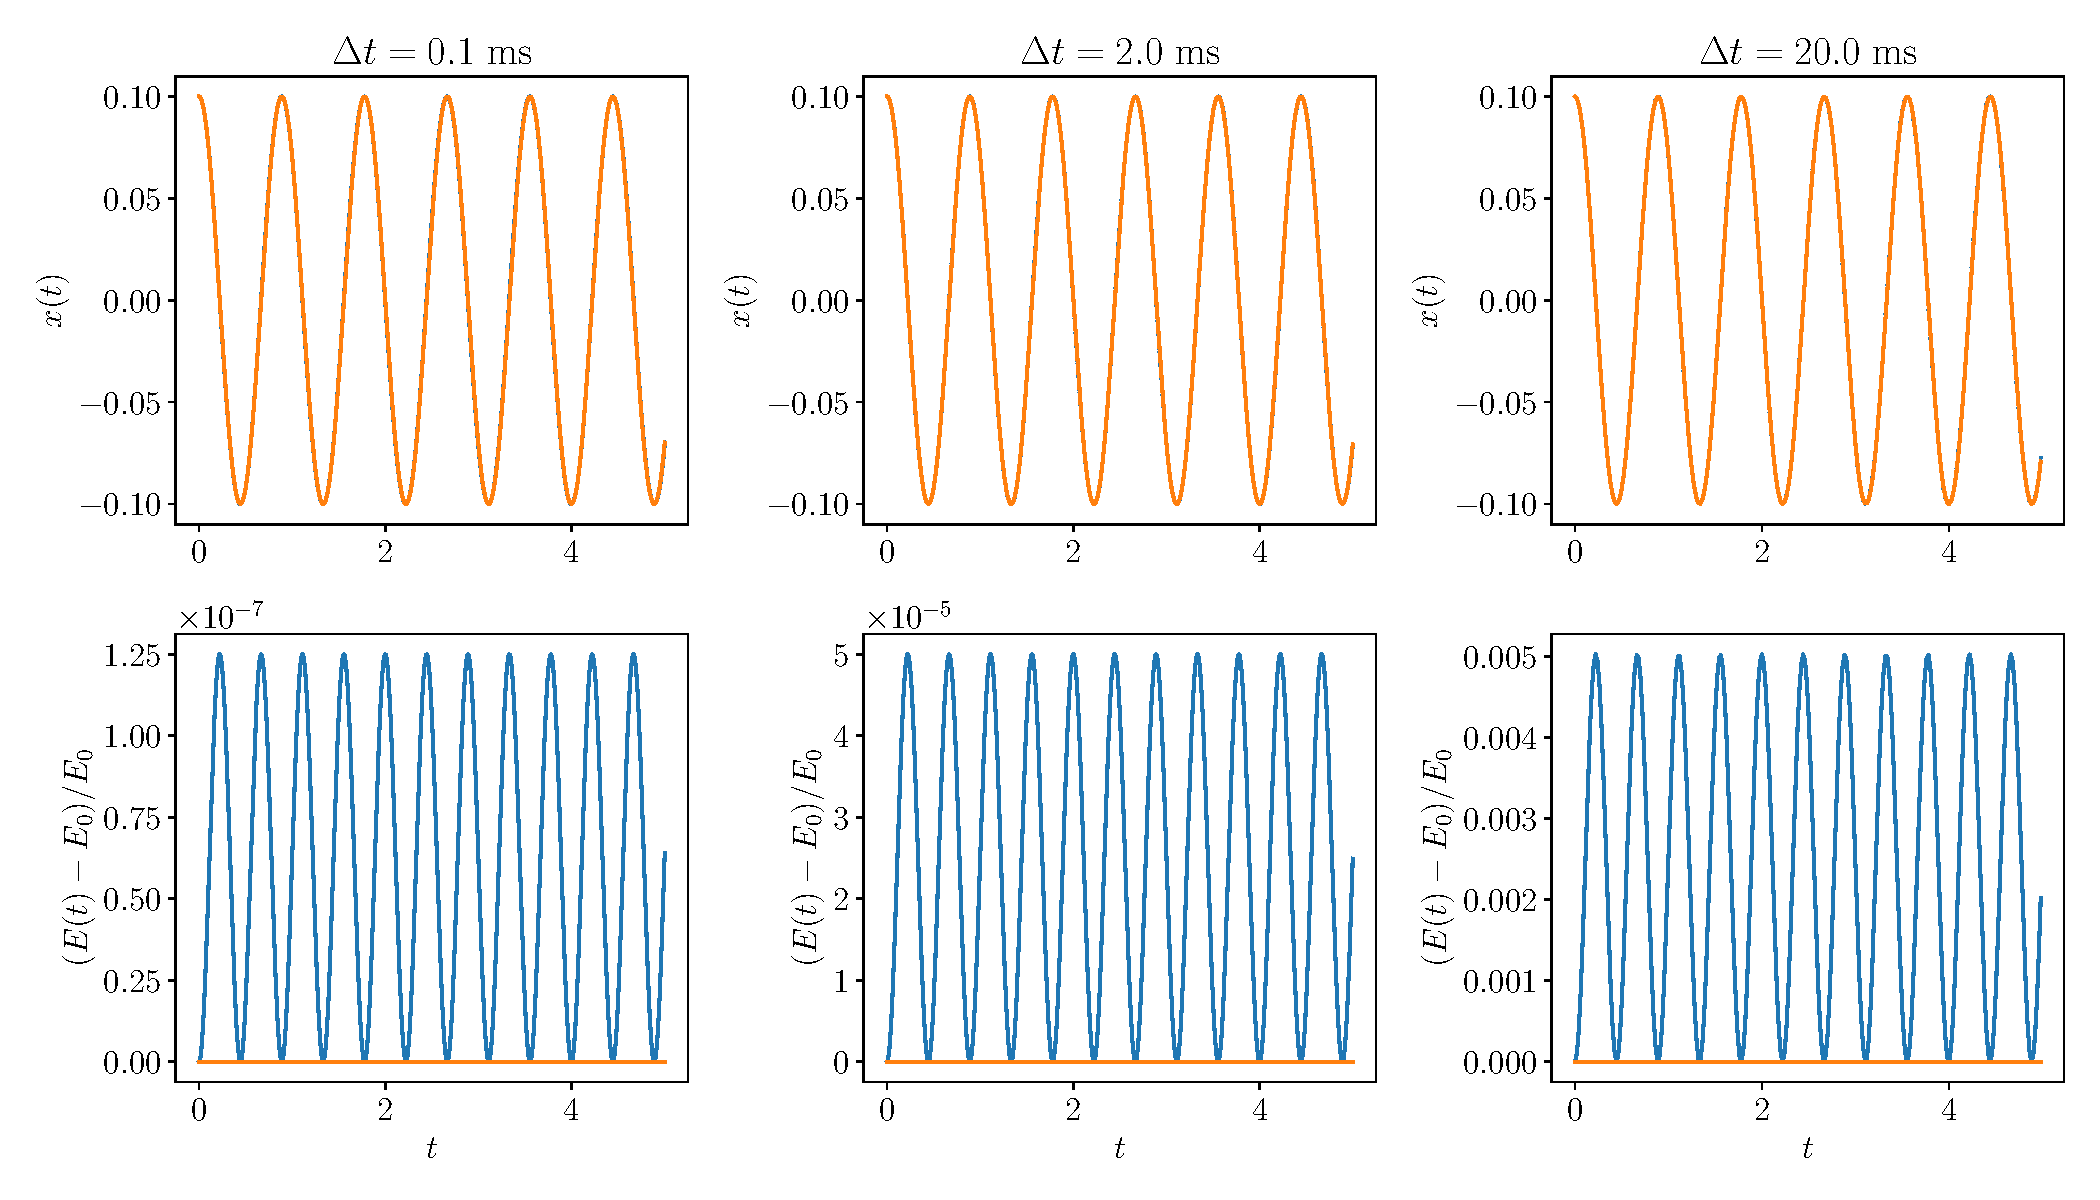
\includegraphics[width=\textwidth]{../Harmonic-Oscillator/figures/leapfrog.pdf}
    \caption{Plots arranged according as in figure \ref{fig:euler_results} except the blue dots being the leapfrog results.}
    \label{fig:leapfrog_results}
\end{figure}

\section*{Excercise 1.6}

\subsection*{a)}
The code for this excercise is shown at the end of the report. It uses the same integrator code as previously, with the force function switched out. Now it uses force derived from a Lennard-Jones potential. Of course this severely impacts the programs performance as the time complexity of simulation $n$ bodies interacting with every other body has the asymptotic time complexity $O(n^2)$. Luckily the interactions obey Newton's 3st law. The force excerted on particle $i$ onto particle $j$ is indentical in size but opposite in direction to the force from $j$ onto $i$. This means that we can eliminate some duplicate calculations through a triangular iteration, resulting in a complexity of $O(n(n+1)/2)$. Some additional speed up can be achieved when calculating the Lennard-Jones potential. There's no need to take the square root of $\sqrt{(\vec{r}_i - \vec{r}_j)^2} = |\vec{r}_i - \vec{r}_j|$ since it'll be raised to the power of 12 or 6 later. Skipping the root calculation and raising it to the power of 6 and 3 instead saves an expensive calculation which is made for every pair of particles.

When plotting, only a tenth or so of the time steps are saved to be drawn. The need for a small $\Delta t$ is only vital to ensure conservation of energy, not to view the process with an adequate resolution.

\subsection*{b)}
Trying different values of $\Delta t$ seems to indicate that about $\sigma/(2v_0) \cdot 0.02$ is about the biggest it can be while still conserving total energy.

\subsection*{c)}
\subsection*{d)}

\end{document}
